\section{Búsqueda sistemática de hiperparámetros}

\subsection{Diseño experimental y tracking en W\&B}

Para la fase 2 se diseñaron tres sweeps independientes en W\&B, uno por modelo, con \textbf{optimización bayesiana}.
La razón de mantener sweeps separados por modelo, en lugar de un único sweep combinado, es preservar la capacidad comparativa: al tener el mismo presupuesto de ejecuciones para cada arquitectura, ningún modelo queda infrarrepresentado en la búsqueda. Esto permite afirmar que el ranking final refleja el potencial real de cada enfoque bajo una exploración equivalente, y no un sesgo introducido por haber buscado más en unos que en otros.

Se ejecutaron \textbf{12 runs por modelo} (36 en total), con semilla fija (42).

Cada run sigue la convención de nombres \texttt{\{modelo\}\_lr\{lr\_head\}\_wd\{wd\}\_unfreeze\{n\}\_\{optim\}} y se etiqueta con el modelo correspondiente para facilitar el filtrado en W\&B. Por cada run se registraron: \texttt{train/loss}, \texttt{val/loss}, \texttt{val/acc} y \texttt{val/f1\_macro} por época, el tiempo por época, la configuración completa de hiperparámetros y el mejor checkpoint. Al finalizar, se guarda la matriz de confusión sobre el conjunto de validación para el checkpoint restaurado.

El espacio de búsqueda fue el mismo para los tres modelos:

\begin{itemize}\setlength\itemsep{2pt}
    \item \textbf{lr\_head}: log-uniforme en $[10^{-4},\,10^{-2}]$; \quad \textbf{lr\_backbone}: log-uniforme en $[10^{-6},\,10^{-4}]$.
    \item \textbf{optimizer}: AdamW o SGD (momentum 0.9); \quad \textbf{weight\_decay}: $\{0.001,\,0.01,\,0.05,\,0.1\}$.
    \item \textbf{unfreeze\_layers}: $\{0,\,1,\,2,\,3\}$ bloques finales del backbone.
    \item \textbf{warmup\_epochs}: $\{3,\,5\}$; \quad \textbf{finetune\_epochs}: $\{5,\,8,\,10\}$.
\end{itemize}

\subsection{Resultados del sweep}

La Figura~\ref{fig:training-curves} muestra la evolución de la accuracy de validación por época para el mejor run de cada modelo. La Tabla~\ref{tab:sweep-resultados} recoge la mejor configuración encontrada.

\begin{figure}[H]
    \centering
    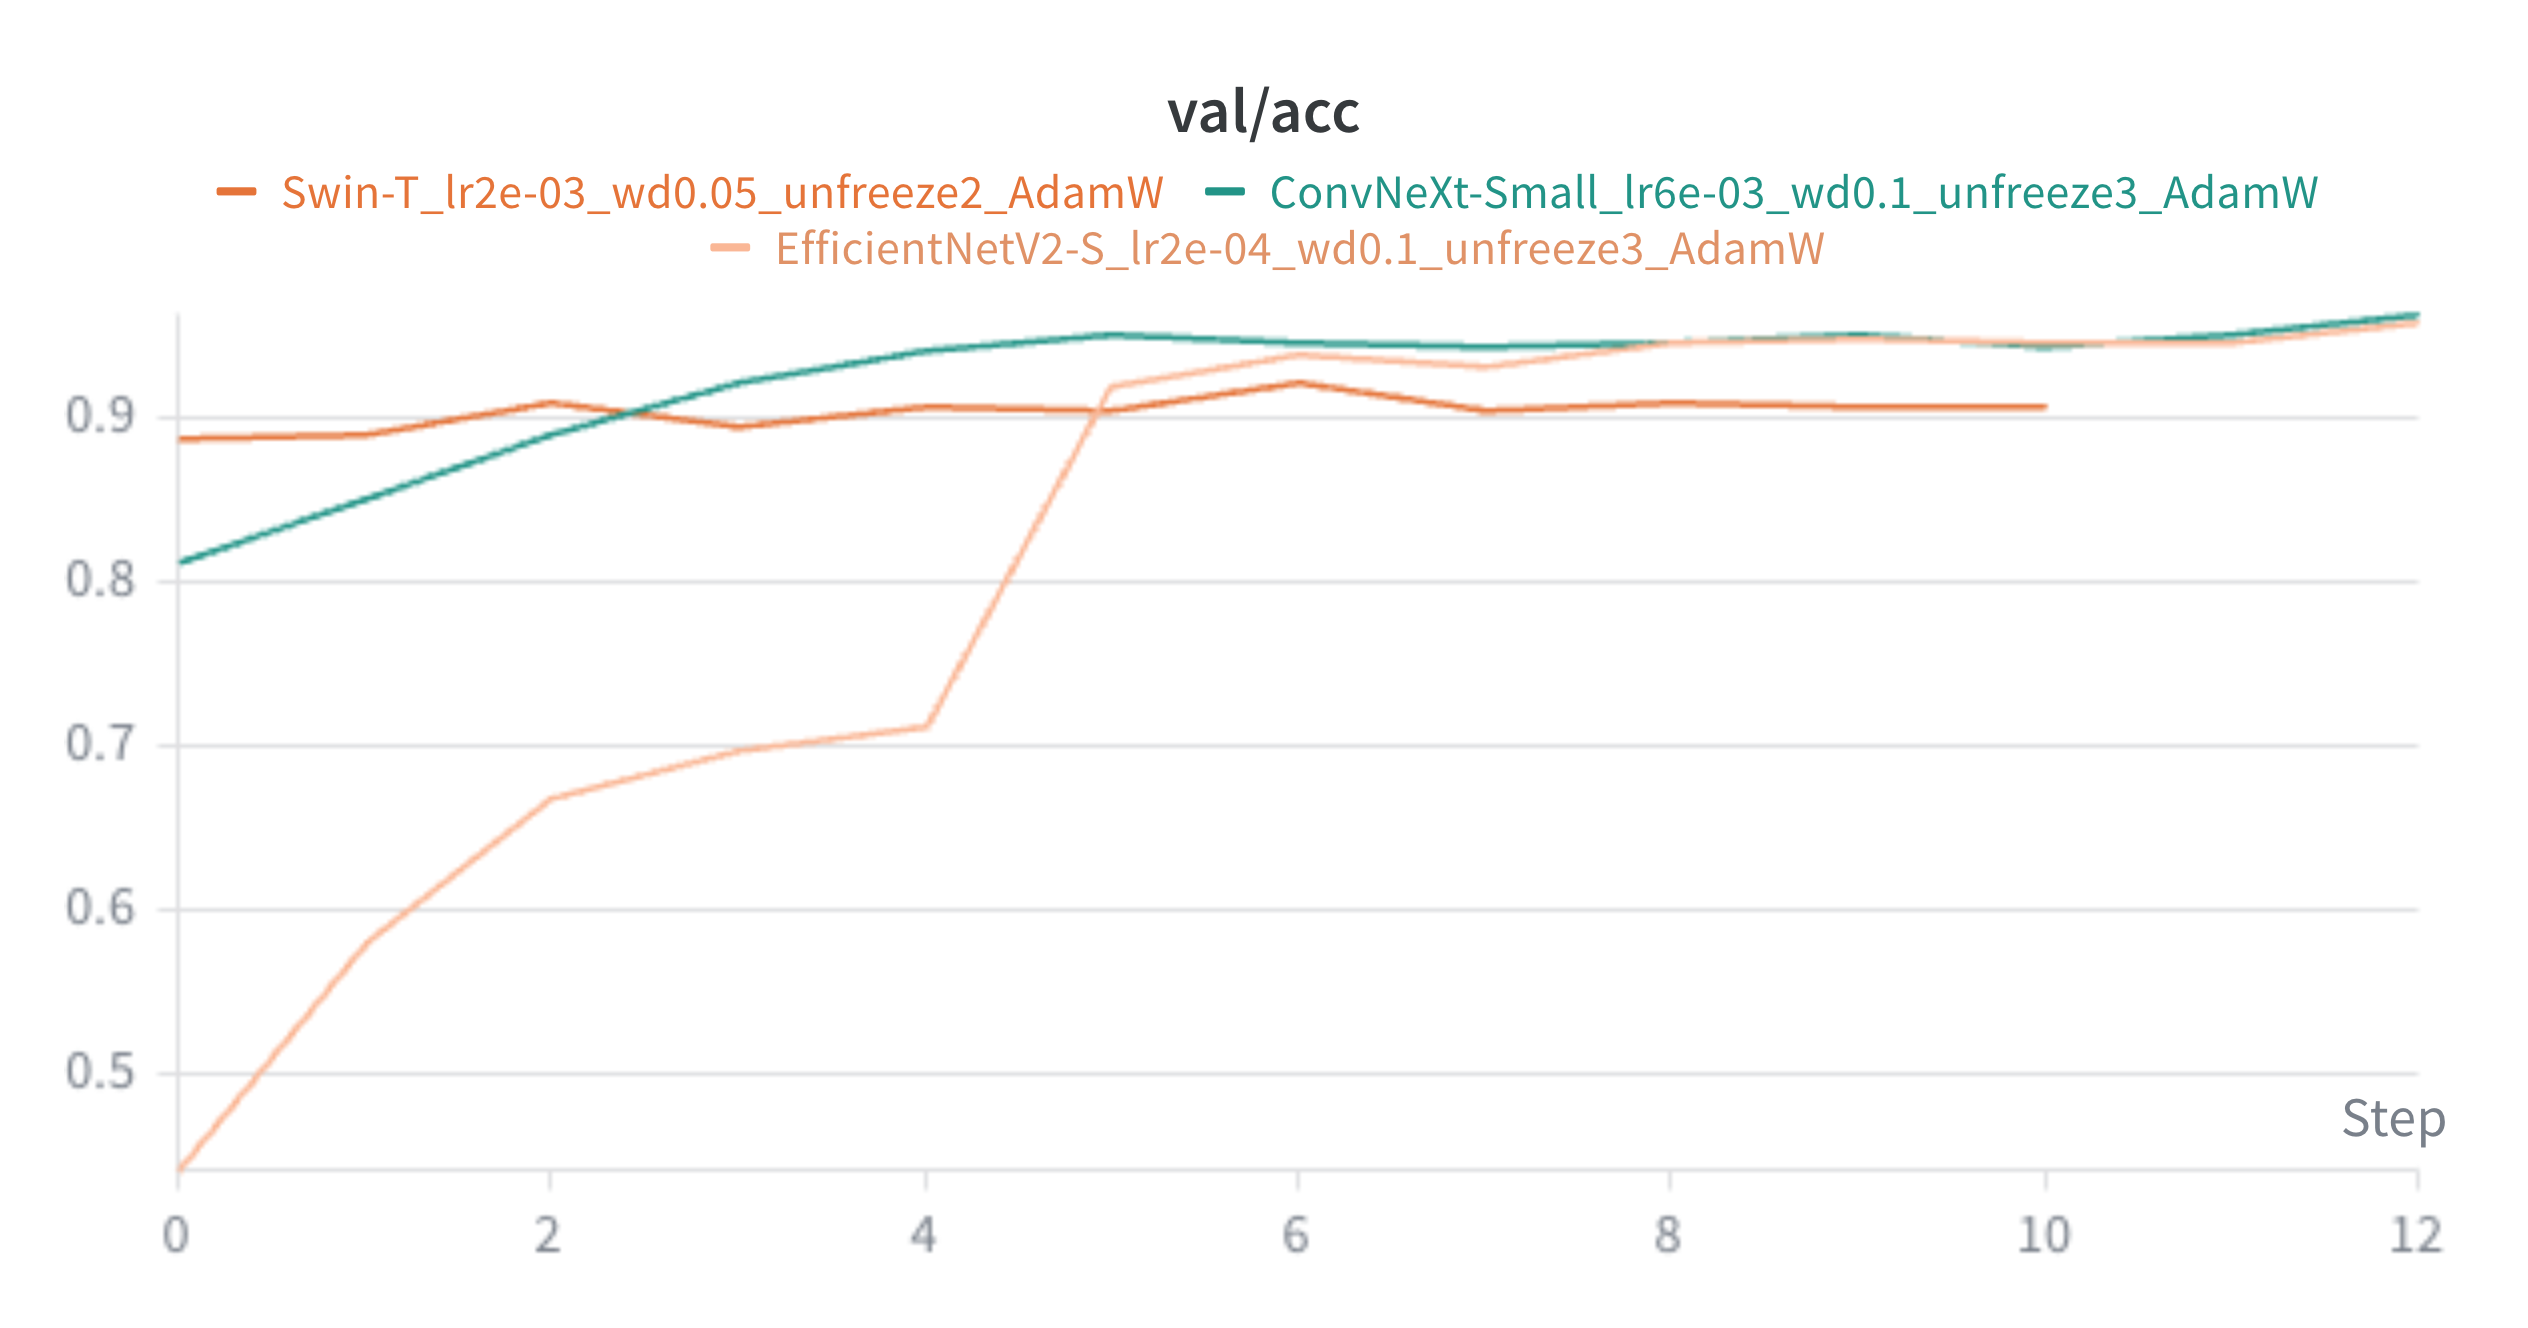
\includegraphics[width=0.82\linewidth]{imagenes/training_curves.png}
    \caption{Curvas de val/acc por época para el mejor run de cada modelo.}
    \label{fig:training-curves}
\end{figure}

La Tabla~\ref{tab:top-runs} muestra los cinco mejores runs por modelo para ilustrar la profundidad de la búsqueda y la estabilidad de las configuraciones ganadoras.

\begin{table}[H]
    \centering
    \caption{Mejor configuración y métricas finales por modelo (36 runs totales).}
    \label{tab:sweep-resultados}
    \begin{tabular}{lcccccc}
        \toprule
        Modelo & Val Acc & F1 Macro & s/época & Optim. & lr\_head & Unfreeze \\
        \midrule
        ConvNeXt-Small    & \textbf{96.47\%} & \textbf{96.47\%} & 99.9 & AdamW & $6.4\!\times\!10^{-3}$ & 3 \\
        EfficientNetV2-S  & 96.00\%          & 96.00\%          & 43.5 & AdamW & $1.8\!\times\!10^{-4}$ & 3 \\
        Swin-T            & 92.27\%          & 92.21\%          & 26.6 & AdamW & $2.4\!\times\!10^{-3}$ & 2 \\
        \bottomrule
    \end{tabular}
\end{table}

\begin{table}[H]
    \centering
    \caption{Top 5 runs por modelo (val\_acc descendente).}
    \label{tab:top-runs}
    \begin{tabular}{llccc}
        \toprule
        Modelo & Configuración & Val Acc & F1 Macro & Optim. \\
        \midrule
        ConvNeXt-S & lr=6.4e-3, wd=0.1, unfreeze=3, ft=10 & 96.47\% & 96.47\% & AdamW \\
                   & lr=6.3e-3, wd=0.1, unfreeze=3, ft=10 & 96.13\% & 96.12\% & AdamW \\
                   & lr=6.0e-3, wd=0.1, unfreeze=3, ft=10 & 95.93\% & 95.93\% & AdamW \\
                   & lr=2.0e-3, wd=0.05, unfreeze=3, ft=10 & 95.87\% & 95.85\% & AdamW \\
                   & lr=1.0e-2, wd=0.05, unfreeze=3, ft=10 & 92.67\% & 92.74\% & SGD   \\
        \midrule
        EffNetV2-S & lr=1.8e-4, wd=0.1, unfreeze=3, ft=8  & 96.00\% & 96.00\% & AdamW \\
                   & lr=5.2e-4, wd=0.1, unfreeze=3, ft=8  & 96.00\% & 96.01\% & AdamW \\
                   & lr=5.1e-4, wd=0.05, unfreeze=3, ft=8 & 95.67\% & 95.67\% & AdamW \\
                   & lr=2.0e-4, wd=0.05, unfreeze=2, ft=5 & 95.07\% & 95.06\% & AdamW \\
                   & lr=2.0e-4, wd=0.05, unfreeze=3, ft=5 & 94.60\% & 94.60\% & AdamW \\
        \midrule
        Swin-T     & lr=2.4e-3, wd=0.05, unfreeze=2, ft=8 & 92.27\% & 92.21\% & AdamW \\
                   & lr=7.9e-3, wd=0.05, unfreeze=2, ft=8 & 92.13\% & 92.12\% & AdamW \\
                   & lr=1.7e-3, wd=0.01, unfreeze=1, ft=5 & 92.13\% & 92.08\% & AdamW \\
                   & lr=2.4e-3, wd=0.05, unfreeze=2, ft=8 & 92.00\% & 91.95\% & AdamW \\
                   & lr=1.2e-3, wd=0.01, unfreeze=1, ft=8 & 92.00\% & 91.94\% & AdamW \\
        \bottomrule
    \end{tabular}
\end{table}

\subsection{Patrones observados}

\textbf{Optimizador:} AdamW dominó en los tres modelos de forma consistente. Los runs con SGD obtuvieron resultados notablemente peores en todos los casos (hasta $-17$ pp en ConvNeXt-Small). La capacidad de AdamW de adaptar la tasa de aprendizaje por parámetro resulta especialmente ventajosa en fine-tuning de redes profundas preentrenadas, donde distintas capas requieren magnitudes de actualización muy diferentes.

\textbf{Capas descongeladas:} \textit{unfreeze=3} fue óptimo para ConvNeXt-Small y EfficientNetV2-S; Swin-T convergió mejor con \textit{unfreeze=2}. Las configuraciones con \textit{unfreeze=0} (solo cabeza, sin fine-tuning) mostraron una caída pronunciada de rendimiento (40--80 pp), confirmando que el fine-tuning parcial del backbone es imprescindible para adaptar las representaciones a nuestro problema.

\textbf{Regularización:} weight\_decay $\geq 0.05$ con AdamW produjo sistemáticamente los mejores modelos, especialmente combinado con learning rates moderados o altos. Una regularización más fuerte controla el sobreajuste que aparece al descongelar capas del backbone con datos de entrenamiento relativamente limitados (2\,985 imágenes).

\textbf{Estabilidad:} Swin-T mostró mayor consistencia entre runs (rango 88\%--92\%), mientras que ConvNeXt-Small y EfficientNetV2-S presentaron mayor varianza ($\sim$15 pp de rango), siendo muy sensibles al optimizador y al número de capas descongeladas.

\textbf{Inversión del ranking:} en el baseline, Swin-T lideraba con 91.1\%. Tras el sweep, ConvNeXt-Small y EfficientNetV2-S lo superan claramente (96\% vs. 92\%), evidenciando que estas arquitecturas tienen mayor capacidad potencial que solo se activa con fine-tuning de capas superiores.
